In this section we describe what the Balloon Server does and how it fits in the
project. 

\subsection{Specifications}

The goal of the Balloon Server is to make users believe that, no matter how
many screens are used for display, there is only one Balloon application. One
way to achieve this is to make the screens look `connected'. That is, after
pushing a balloon through the left edge of a screen, the balloon should
reappear at the right edge of another screen. Another way is to enforce that a
balloon is shown only on one screen at any given time.

We want users to believe that the balloon that appeared in one screen is the
same balloon that disappeared in the other screen. Since the appearance of
balloons is customisable (the colour and texture can be changed by the user),
believing they are the same is easier if customisations are kept when
transferring the balloon from one screen to another. In addition, it is more
believable if balloons keep their speed and direction when moving across 
screens.

The server is responsible for notifying the client when balloons should appear
on its screen and how (e.g. what type of balloon, caption text, content
to show when popping the balloon). The server does not create the data needed to
display balloons itself. This task is the responsibility of the Web Feed. In
order to have balloons to provide to the client, the server has to regularly
retrieve the information needed to create these balloons from the feed.

Something to keep in mind is that the content of this feed changes with time
(i.e. new items are added from the Twitter aggregator and user-submitted 
content) but we want to keep the number of balloons on each screen at a
reasonable level. This is why the server has to decide which balloons should be
kept and which should be discarded when new items are retrieved from the feed.
We have decided to discard all balloons without a corresponding feed item.

An additional requirement is that the number of screens connected to the server
is not fixed and can change over the lifetime of the server execution. This
means that connecting and disconnecting screens from the server can be done at
any time and will not halt or impair the processing of balloons. For example, 
when a screen is added the server requests more items from the feed. These new
items are used to create new balloons to populate the new, empty screen. When 
disconnecting a screen, its balloons are transferred to the remaining screens.

Late in the project, we decided to introduce on-screen `tips' to help new users
interact with our application. This was materialised as a plane carrying a label
showing the tip banner behind it. The server is responsible for deciding when 
such planes are shown, transferring them between screens and deciding when they
have to disappear. Indeed we felt that always having a plane on a screen could
be annoying for the users, especially since planes can collide with balloons 
and push them away when users might be interacting with them.

\clearpage{}
\subsection{Design}

As the server is a self-contained part of the project, we have decided to 
develop it as a separate program. This allowed us to have clear interfaces 
between the server and other parts of the project and made it easier for
multiple people to work on different parts of the project at the same time.
Most of the communication happens between the client and the server, which 
meant that writing the server in the same language than the client (C\#) let us 
share much code between the two and let the client team focus on client issues 
and not network issues.

The server communicates with the feed through the standard HTTP protocol 
(using JSON to format feed data) and with the Balloon Client through a custom 
protocol that is used over TCP/IP sockets. The former choice was decided by the 
Web team and motivated by ease of use and reuse of existing libraries. As far 
as we are aware there is no existing protocol that lets coordinating content
balloons over different screens, therefore we had to create our own. Using 
sockets instead of leveraging higher-level communication frameworks was chosen 
to make debugging easier by writing explicit code at the expense of writing 
more code.

\subsubsection{Messaging}

There is in general two ways to communicate between two applications: messaging 
and Remote Procedure Call. We have chosen the former as we have some experience 
with it. We also believe it is easier to design a networked application when 
requests and responses are represented and passed around explicitly (e.g. as 
messages). In particular, the messaging approach makes it easier (and obvious) 
in which thread a message is processed. This is especially important in the 
client where drawing the game must be done in a special thread.

With a messaging approach, the interface between client and server is defined by 
a set of messages that can be sent by one or the other or both (see figures 
\ref{ServerMessages}, \ref{ClientMessages} and \vref{CommonMessages}). The most
important messages are NewBalloon/PopObject (they control balloons appearing/
disappearing on the screen) and ChangeScreen (controls balloons moving between
screens).

\begin{table}
\begin{tabular}{|>{\raggedright}p{4.3cm}|>{\raggedright}p{2.8cm}|>{\raggedright}p{8.7cm}|}
\hline 
Message Name & Parameters & Description\tabularnewline
\hline 
NewBalloon
& Balloon ID 
\newline Direction
\newline Position (Y)
\newline Velocity (X, Y)
& A new balloon should appear on the screen at the given screen height (Y position),
with the given direction and on the side of the screen given by the direction.
\tabularnewline
\hline 
NewPlane
& Plane ID 
\newline Plane type
\newline Direction
\newline Position (Y)
\newline Velocity (X, Y)
\newline Time
& A new plane should appear on the screen at the given screen height (Y position),
with the given direction, on the side of the screen given by the direction, with
a message given by its type and with the specified initial animation time.
\tabularnewline
\hline 
BalloonContentUpdate
& Balloon ID 
\newline Balloon type
\newline Label
\newline Content
\newline URL
\newline Image URL
& Indicates that the content of the specified balloon (caption label, content
text to display when the balloon is popped, URL to the article, URL to the image) 
has been changed. 
\tabularnewline
\hline 
\end{tabular}

\caption{Messages sent by the server}

\label{ServerMessages}
\end{table}

\begin{table}
\begin{tabular}{|>{\raggedright}p{4.3cm}|>{\raggedright}p{2.8cm}|>{\raggedright}p{8.7cm}|}
\hline 
Message Name & Parameters & Description\tabularnewline
\hline 
ChangeScreen
& Balloon ID 
\newline Direction
\newline Position (Y)
\newline Velocity (X, Y)
\newline Time
& The given balloon or plane moved off the screen at the given screen height (Y position),
with the given direction and on the side of the screen given by the direction. For planes,
the time value is the current animation time.
\tabularnewline
\hline 
GetBalloonContent
& Balloon ID
& Request that the content of the specified balloon be sent to the client.
\tabularnewline
\hline 
GetBalloonState
& Balloon ID
& Request that the state of the specified balloon be sent to the client.
\tabularnewline
\hline 
\end{tabular}

\caption{Messages sent by the client}

\label{ClientMessages}
\end{table}

\begin{table}
\begin{tabular}{|>{\raggedright}p{4.3cm}|>{\raggedright}p{2.8cm}|>{\raggedright}p{8.7cm}|}
\hline 
Message Name & Parameters & Description\tabularnewline
\hline 
PopObject
& Balloon ID or plane ID
& When sent by the client, indicates that the user popped the specified balloon.
When sent by the server, indicates that the specified balloon or plane has been 
removed from the screen (after updating the feed).
\tabularnewline
\hline 
BalloonStateUpdate
& Balloon ID
\newline Overlay type
\newline Background colour
\newline Number of votes
& Indicates that the state of the given balloon (overlay texture, background colour
and number of votes) has been changed. This can be sent by the server when the 
number of votes changes or by the client when the user changes a balloon's 
decoration with paint buckets.
\tabularnewline
\hline 
\end{tabular}

\caption{Messages sent by both client and server}

\label{CommonMessages}
\end{table}

One important aspect of this communication is that it is asynchronous. This 
means that messages are sent as a kind of notification to the recipient. The 
sender does not wait for a `return receipt' from the recipient before resuming 
its activity. Indeed in general it does not need to know when the message has
arrived. The only exception comes with the GetBalloonContent/GetBalloonState 
messages which are answered by BalloonContentUpdte/BalloonStateUpdate messages.
Howerver, the latter messages can be also sent spontaneously (e.g. when the user 
changes a balloon's decoration using the paint buckets). Messages are handled 
the same no matter if they are spontaneous or a response from another message.

Sockets can only send and receive bytes. This is why there must be a way to
transform message objects from and to bytes, in order to transmit them over the
networks between the screens and server. This process is called serialisation. 
During this project we have implemented two serialisation formats. The first is
a text-based format based on JSON and was used for the first prototypes of our 
project. Text-based formats are usually very flexible and easy to debug; on
the other hand they are quite slow to manipulate. This is why a second, binary
serialiser was written after the first prototypes were successful.


\subsubsection{Architecture}

The main reason from shying away from communication frameworks and libraries was
to be able to easily change the architecture (in particular, threading) of the 
server if the need arose. Possible issues that come with a bad threading design 
include non-intuitive behaviour; subtle, difficult-to-reproduce bugs and low 
performance. This is why it was important to have a good architecture to avoid 
these issues as much as possible. We had to change it multiple times during the 
course of this project when we ran into some of these issues.

\begin{figure}
\begin{centering}
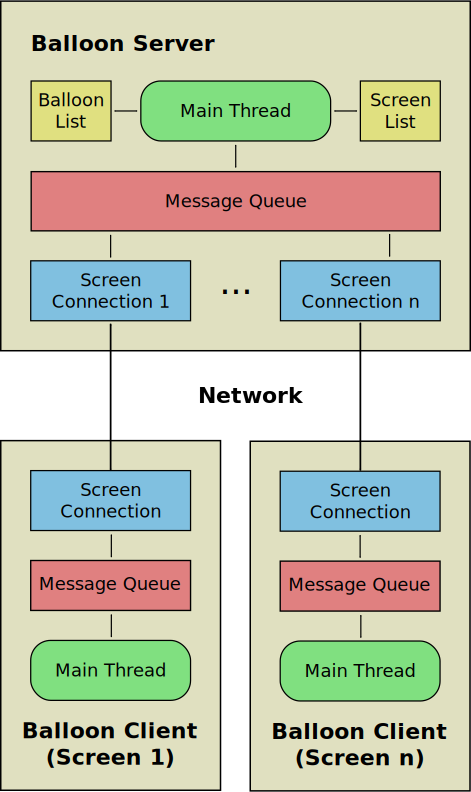
\includegraphics[scale=0.95]{Diagrams/messaging}
\par\end{centering}

\caption{Messaging and Threading Architecture}
\label{Messaging-Arch}
\end{figure}

The final architecture (see figure \vref{Messaging-Arch}) tries to minimise the
use of threads. In particular, in both client and server, as much processing as
possible is done in a single thread (`Main thread' for the server, `GUI thread'
for the client). However, messages received over the network
can arrive in any thread (this is because we are using asynchronous I/O). To 
keep all processing on the main thread, these messages are placed in a thread-safe
message queue and then removed in order by the main thread when it is ready. 

This design pattern (thread with a message/event loop) is used throughout the
application. In the client, the GUI thread has a message queue which it empties
during the `Update' phase. In the server, both the main thread and feed reader 
thread have a message queue; they communicate by placing messages in each other's
queue. This approach limits the need for synchronisation between threads and 
thus avoids associated pitfalls.

The reason we have a separate thread for the feed reader is that pulling the 
feed can take a long time (several seconds). If this was done on the main 
thread, during this time the server would be blocked (e.g. balloons would not 
reappear on another screen after moving out of one screen) which we wanted to 
avoid. With this approach, the feed reader thread is blocked when updating the
feed while the main thread can continue processing. When the update is done, the
new feed items are placed in the message queue and processed by the main thread.
Similarly in the client, long-running operations such as downloading images and 
rendering HTML pages are done on a background thread and the result is used in 
the GUI thread.

\clearpage{}
\subsection{Persistence}

By persistence, we mean saving the balloon data manipulated by the server between 
executions. Persisting balloon data means that when shutting down the 
server and then starting it again this data would be preserved. Since it 
originates from the feed and can be re-queried at will, we have chosen not to
have any persistence for balloon data. However, some data is persisted across 
execution as we will see in the next section about configuration.

Even though we have made this choice, this does not mean persistence could not 
be implemented for this project in the future. The serialisation and message 
classes we wrote to support communication between client and server could be 
reused fairly easily to this end (e.g. serialising messages to a buffer and 
then writing this buffer to a file).

\subsection{Configuration}

This part of the application was at the beginning only intended to be used by 
the server but was later extended to the client as well. It puts together many 
variables that change the behaviour of the application (e.g. how many balloons 
to show on each screen, which URL to query the feed from, how often it  
should be queried, etc). The value of these variables can be written to or read 
from a file by the application. We have chosen the JSON format for such files, 
which is easily manipulated with a text editor. When the server (or client) is 
started and this file does not exist, a file containing default values for the 
variables is created.

